% THIS DOCUMENT IS FOLLOWS THE VOLERE TEMPLATE BY Suzanne Robertson and James Robertson
% ONLY THE SECTION HEADINGS ARE PROVIDED
%
% Initial draft from https://github.com/Dieblich/volere
%
% Risks are removed because they are covered by the Hazard Analysis
\documentclass[12pt]{article}

\usepackage{booktabs}
\usepackage{tabularx}
\usepackage{longtable}
\usepackage{graphicx}
\usepackage{hyperref}
\usepackage{float}
\graphicspath{ {./res/} }
\hypersetup{
    bookmarks=true,         % show bookmarks bar?
      colorlinks=true,      % false: boxed links; true: colored links
    linkcolor=red,          % color of internal links (change box color with linkbordercolor)
    citecolor=green,        % color of links to bibliography
    filecolor=magenta,      % color of file links
    urlcolor=cyan           % color of external links
}

\newcommand{\lips}{\textit{Insert your content here.}}

%% Comments

\usepackage{color}

\newif\ifcomments\commentstrue %displays comments
%\newif\ifcomments\commentsfalse %so that comments do not display

\ifcomments
\newcommand{\authornote}[3]{\textcolor{#1}{[#3 ---#2]}}
\newcommand{\todo}[1]{\textcolor{red}{[TODO: #1]}}
\else
\newcommand{\authornote}[3]{}
\newcommand{\todo}[1]{}
\fi

\newcommand{\wss}[1]{\authornote{blue}{SS}{#1}} 
\newcommand{\plt}[1]{\authornote{magenta}{TPLT}{#1}} %For explanation of the template
\newcommand{\an}[1]{\authornote{cyan}{Author}{#1}}

%% Common Parts

\newcommand{\progname}{ProgName} % PUT YOUR PROGRAM NAME HERE
\newcommand{\authname}{Team \#, Team Name
\\ Student 1 name
\\ Student 2 name
\\ Student 3 name
\\ Student 4 name} % AUTHOR NAMES                  

\usepackage{hyperref}
    \hypersetup{colorlinks=true, linkcolor=blue, citecolor=blue, filecolor=blue,
                urlcolor=blue, unicode=false}
    \urlstyle{same}
                                


\begin{document}

\title{Software Requirements Specification for \progname: subtitle describing software} 
\author{\authname}
\date{\today}
	
\maketitle

~\newpage

\pagenumbering{roman}

\tableofcontents

~\newpage

\section*{Revision History}

\begin{tabularx}{\textwidth}{p{3cm}p{2cm}X}
\toprule {\textbf{Date}} & {\textbf{Version}} & {\textbf{Notes}}\\
\midrule
Date 1 & 1.0 & Notes\\
Date 2 & 1.1 & Notes\\
\bottomrule
\end{tabularx}

~\\

~\newpage
\section{Purpose of the Project}
\subsection{User Business}

With the world currently facing record high inflation, cost-of-living is at the highest
it has ever been. This affects all daily necessities but is especially true for food and groceries.
As a whole, all households are affected but there is particular financial strain on those with lower-incomes.
As a result, interest in personal finance has grown and become more important in peoples' everyday lives.
To assist these individuals, we are developing an application that can help users better understand their
spending habits and make smarter financial decisions. This application will allow users to
take photos of grocery receipts and track their overall spending, analyze spending trends, and receive
suggestions on cheaper alternatives for purchased grocery items. Overall, we believe this application
will help users stay more informed and reduce grocery spending in the long-term.

\subsection{Goals of the Project}
\begin{itemize}
  \item The created application will help users save money on groceries over time.
  \item The application will provide accurate spending data and suggestions to end users.
\end{itemize}  
\section{Stakeholders}
\subsection{Client}
Both the client and customer will be the users of the system. These primary stakeholders are made up of low-income households of Hamilton and university students from McMaster who want to save money on groceries. The stakeholders will make decisions that influence the system through surveys, studies, and focus groups.
\subsection{Customer}
Outlined in the above Client section.
\subsection{Other Stakeholders}
\begin{itemize}
  \item Grocery stores in the area
  \item Household members (people who the groceies are being purchased for)
  \item Mobile application store (ios app store, google play store)
  \item Any invidividual who wants to save on groceries
\end{itemize}

\subsection{Hands-On Users of the Project}
Low income households and individuals who are budget constrained on their groceries. The archetypal customer will have access to a device with a camera and have access to the internet. This entails adults or young adults who are responsible for making decisions on grocery items. Customers want to reduce the cost of their grocery items whilst maximizing the convenience of their grocery shopping trip. 
\begin{itemize}
  \item Low or single income households in Hamilton
  \begin{itemize}
    \item Shops for household groceries.
    \item Moderate experience with navigation mobile applications.
    \item 30-70 years of age.
    \item Has vehicle or some means to travel.
  \end{itemize}
  \item Students of McMaster University
  \begin{itemize}
    \item Shops for individual groceries
    \item Adept experience with navigation mobile applications.
    \item 20-30 years of age.
    \item Has no vehicle or limited means to travel.
  \end{itemize}
\end{itemize}

\subsection{Personas}
\begin{itemize}
  \item John Bertuzzi
  \begin{itemize}
    \item Age: 22
    \item Favorite food: Chicken and Pasta
    \item Nursing Student at McMaster University
    \item Living in Ainslie Wood East.
    \item Athlete.
    \item Missing teeth.
  \end{itemize}
  \item Alice Woll
  \begin{itemize}
    \item Age: 51
    \item Favorite food: Grilled Cheese
    \item Mother of 2, Spouse of William Woll.
    \item Accountant for tech company.
    \item Living in Westdale.
    \item Likes to watch Hockey.
  \end{itemize}
\end{itemize}

\subsection{Priorities Assigned to Users}
All users will have equal priority within the system.

\subsection{User Participation}
Everyday users will provide their shopping data to the community database. This will be of no additional time commitment than they are already required to use the system at a base level.

From an elicitation perspective, a sample of users will be responsible for providing usability, look, and feel requirements feedback. This will be done at various stages in development.
\subsection{Maintenance Users and Service Technicians}
*** N/A

\section{Mandated Constraints}
\subsection{Solution Constraints}
\lips
\subsection{Implementation Environment of the Current System}
\lips
\subsection{Partner or Collaborative Applications}
\lips
\subsection{Off-the-Shelf Software}
\lips
\subsection{Anticipated Workplace Environment}
\lips
\subsection{Schedule Constraints}
\lips
\subsection{Budget Constraints}
\lips
\subsection{Enterprise Constraints}
\lips

\section{Naming Conventions and Terminology}
\subsection{Glossary of All Terms, Including Acronyms, Used by Stakeholders
involved in the Project}
\lips

\section{Relevant Facts And Assumptions}
\subsection{Relevant Facts}
\lips
\subsection{Business Rules}
\lips
\subsection{Assumptions}
\lips

\section{The Scope of the Work}
\subsection{The Current Situation}
\begin{figure}[H]
    \centering
    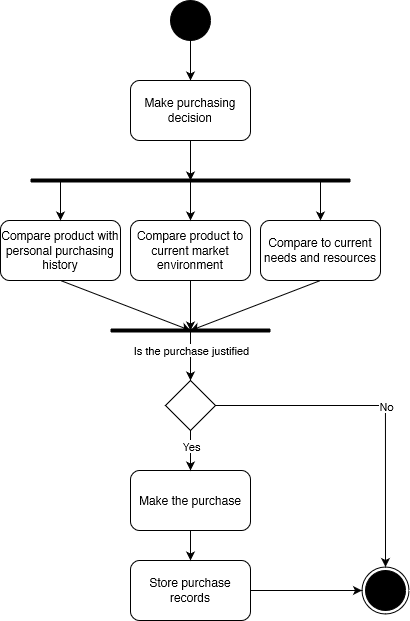
\includegraphics[width=0.6\textwidth]{currentsituation}
    \caption{Current Situation Activity Diagram}
    \label{fig:currentsituation}
\end{figure}
\subsection{The Context of the Work}
\begin{figure}[H]
    \centering
    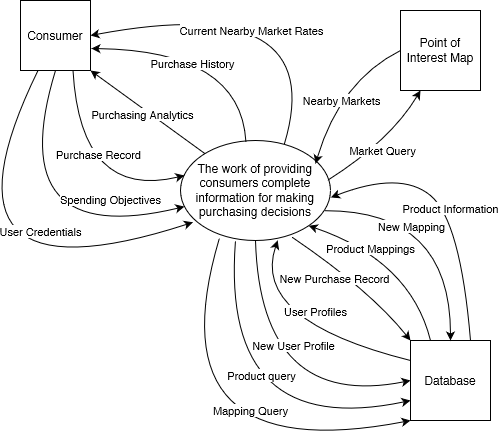
\includegraphics[width=0.9\textwidth]{workcontext}
    \caption{Work Context Model}
    \label{fig:workcontext}
\end{figure}
\subsection{Work Partitioning}
    \begin{longtable}{| >{\raggedright\arraybackslash}p{.30\textwidth} | >{\raggedright\arraybackslash}p{.30\textwidth} | >{\raggedright\arraybackslash}p{.30\textwidth} |}
        \hline
        \textbf{Event Name} & \textbf{Input/output} & \textbf{Summary of BUC} \\
        \hline
        User inputs user profile credentials & User Credentials (in) & Initialize user profile from received credentials \\
        \hline
        Consumer inputs spending objectives & Spending objectives (in) & Records the objectives and the owner \\
        \hline
        Consumer inputs purchase record & Purchase record (in) & Records the purchase and the owner of the purchase \\
        \hline
        User requests purchasing analytics & Purchasing analytics (out) & Report compiled and computed information from available data for the user profile \\
        \hline
        User requests personal purchase history & Purchase history (out) & Report compiled user purchasing history\\
        \hline
        User requests information on a product & Current nearby market rates (out) & Report market rates for a product that is accessible to the user \\
        \hline
        Compiling market information relevant to a user & Nearby markets (in) & Record information for accessible markets based on criteria \\
        \hline
        Request information on markets & Market query (out) & Send request for market information under a set of specified parameters \\
        \hline
        Database transmits product information & Product information (out) & Record information on product \\
        \hline
        New mapping received & Mapping Data (out) & Send new good/service mapping to database \\
        \hline
        Database transmits requested mapping data & Product mappings (in) & Record the product mappings \\
        \hline
        Send purchase record to database & New purchase record (out) &  Send purchase record to database \\
        \hline
        Database transmits requested user profile data & User profiles (in) &  Record the user profile data \\
        \hline
        Send user profile data & New user profile (out) &  Send a user profile to database \\
        \hline
        Send product query to database & Product query (out) & Request relevant data based on product query from database \\
        \hline
        Send mapping query to database  & Mapping query (out) &  Request relevant data based on mapping query from database \\
        \hline 
        \caption{Business Event List}
        \label{tab:businesseventlist}
    \end{longtable}
\subsection{Specifying a Business Use Case (BUC)}
\textbf{Title:} Create a new profile\\
\textbf{Trigger:} User creates a new profile\\
\textbf{Pre-condition:} User has application running\\
\textbf{Outcome: } 
\begin{enumerate}
    \item User creates an profile identified by a username and a password
    \item System creates new profile entry in database
\end{enumerate}
\textbf{Title:} Log in to user profile\\
\textbf{Trigger:} User submits profile credentials \\
\textbf{Pre-condition:} Profile exists in database \\
\textbf{Outcome: } 
\begin{enumerate}
    \item System checks if profile credentials exists
    \item If exists, system allows loads user profile
    \item If not exists, systems shows error message
\end{enumerate}
\textbf{Title:} Record user objectives \\
\textbf{Trigger:} User submits personal objectives \\
\textbf{Pre-condition:} User is logged into profile \\
\textbf{Outcome: } 
\begin{enumerate}
    \item System stores user budgeting objectives of budget with associated product or product groups
\end{enumerate}
\textbf{Title:} Input purchase records \\
\textbf{Trigger:} User submits image or manual entry of purchase record \\
\textbf{Pre-condition:} User is logged into profile \\
\textbf{Outcome: } 
\begin{enumerate}
    \item System reads and translates records to Strings
    \item System maps input records to database objects
    \item If mapping does not exist, make guesses and prompt user for feedback
    \item Save records to database
\end{enumerate}
\textbf{Title:} Create new mapping feedback \\
\textbf{Trigger:} Product mapping is not found in database \\
\textbf{Pre-condition:} Product record has been submitted \\
\textbf{Outcome: } 
\begin{enumerate}
    \item Create mapping guesses using language model
    \item Prompt user with guesses for feedback
    \item User inputs feedback
    \item Process and screen user feedback
    \item If mapping is eligible, create new mapping entry in database
\end{enumerate}
\textbf{Title:} Create user profile analytics \\
\textbf{Trigger:} User requests purchasing analytics \\
\textbf{Pre-condition:} User is logged into profile \\
\textbf{Outcome: } 
\begin{enumerate}
    \item Retrieve user data from database
    \item Transform user profile data into graphics
    \item Display graphics in application
\end{enumerate}
\textbf{Title:} Retrieve profile purchase history \\
\textbf{Trigger:} User requests purchase history\\
\textbf{Pre-condition:} User is logged into profile\\
\textbf{Outcome: } 
\begin{enumerate}
    \item Retrieve user purchase history from database
    \item Transform user purchase history into graphics
    \item Display graphics in application
\end{enumerate}
\textbf{Title:} Retrieve product information \\
\textbf{Trigger:} User requests product information\\
\textbf{Pre-condition:} User is logged into profile and has current location information set \\
\textbf{Outcome: } 
\begin{enumerate}
    \item Retrieve user purchase history from database relevant to the product
    \item Retrieve markets accessible to the user from map service
    \item Retrieve product information belonging to the accessible markets from database
    \item Transform data into graphics
    \item Display graphics in application
\end{enumerate}
\textbf{Title:} Set location information \\
\textbf{Trigger:} User sets location information \\
\textbf{Pre-condition:} User is logged into profile and location information is available \\
\textbf{Outcome: } 
\begin{enumerate}
    \item User sets initial location
    \item User sets accessibility radius
    \item Information is stored locally on device
\end{enumerate}

\section{Business Data Model and Data Dictionary}
\subsection{Business Data Model}
\begin{figure}[H]
    \centering
    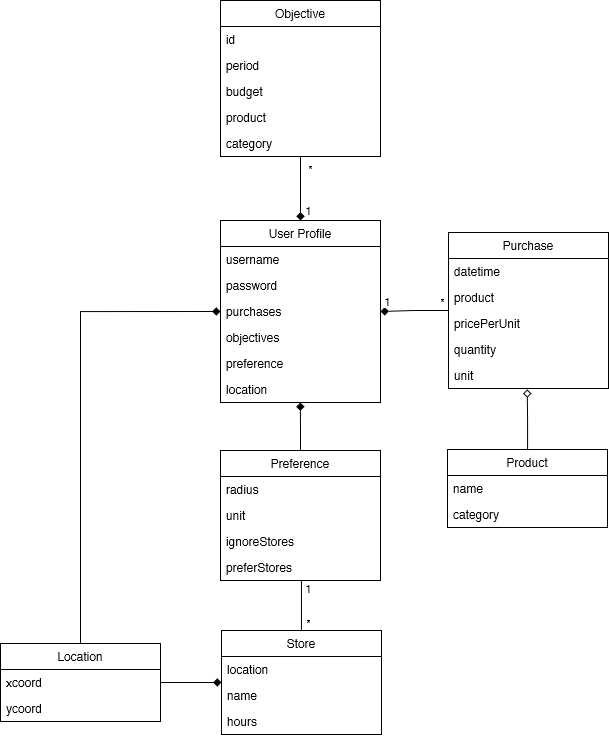
\includegraphics[width=0.85\textwidth]{classdiagram}
    \caption{Class Diagram}
    \label{fig:classdiagram}
\end{figure}
\subsection{Data Dictionary}
\begin{longtable}{| >{\raggedright\arraybackslash}p{.20\textwidth} | >{\raggedright\arraybackslash}p{.55\textwidth} | >{\raggedright\arraybackslash}p{.15\textwidth} |}
        \hline
        \textbf{Name} & \textbf{Content} & \textbf{Type} \\
        \hline
        User Profile & Username + Password + Purchases + Objectives + User Preference + User Location & Class \\
        \hline
        Objective & Objective Id + Period + Budget + Target Product + Target Category & Class \\
        \hline
        Purchase & Datetime + Purchased Product + Price Per Unit + Quantity + Unit & Class \\
        \hline
        Product & Product Name + Category & Class \\
        \hline
        Preference & Accessible Radius + Ignore Stores + Prefer Stores + Prefer Units & Class \\
        \hline
        Store & Store Location + Store Name & Class \\
        \hline
        Location & X-Coordinate + Y-Coordinate & Class \\
        \hline
        Username & *Unique String* & Attribute\\
        \hline
        Password & *String* & Attribute \\
        \hline
        Purchases & *List of Purchase class* & Attribute \\
        \hline
        Objectives & *List of Objective class* & Attribute \\
        \hline
        User Preference & *Preference class* & Attribute \\
        \hline
        User Location & *Location class* & Attribute \\
        \hline
        Objective Id & *String* & Attribute \\
        \hline
        Period & *String: day/week/month/year* & Attribute\\
        \hline
        Budget & *Currency amount measured by Double to 2 decimals* & Attribute \\
        \hline
        Target Product & *String product name* & Attribute \\
        \hline 
        Target Category & *String category name* & Attribute \\
        \hline 
        Datetime & *YYYY-MM-DD HH:MM:SS* & Attribute \\
        \hline 
        Purchased Product & *String Product name* & Attribute \\
        \hline 
        Price Per Unit & *Int price per unit of product* & Attribute \\
        \hline 
        Unit & *String* & Attribute \\
        \hline 
        Quantity & *Double* & Attribute \\
        \hline 
        Product Name & *String* & Attribute \\
        \hline 
        Category & *String* & Attribute \\
        \hline 
        Accessible Radius & *Integer* & Attribute \\
        \hline 
        Ignore Stores & *List of Stores to ignore* & Attribute \\
        \hline 
        Prefer Stores & *List of Stores to prioritise* & Attribute \\
        \hline 
        Prefer Units & *String: metric/imperial* & Attribute \\
        \hline
        Store Location & *Location class* & Attribute \\
        \hline 
        Store Name & *String* & Attribute \\
        \hline 
        X Coordinate & *Double* & Attribute \\
        \hline 
        Y Coordinate & *Double* & Attribute \\
        \hline 
        \caption{Business Event List}
        \label{tab:businesseventlist}
    \end{longtable}

\section{The Scope of the Product}
\subsection{Product Boundary}
\begin{figure}[H]
  \centering
  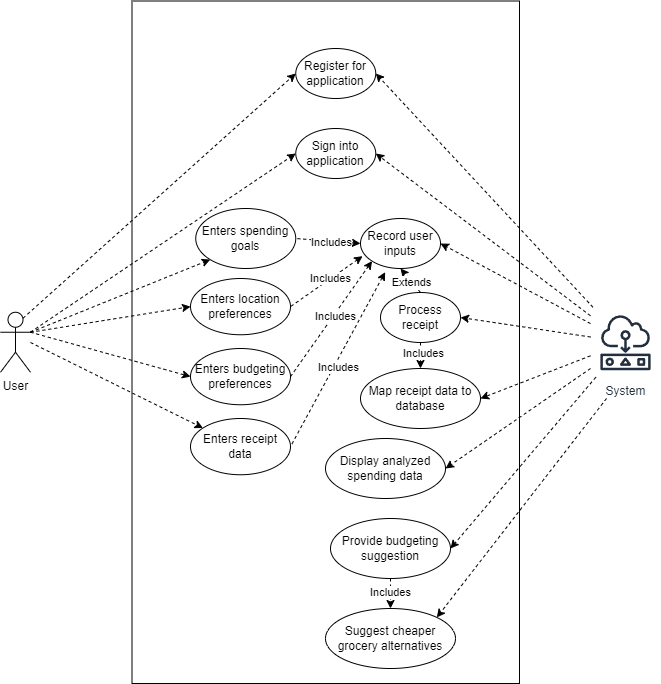
\includegraphics[width=\textwidth]{use_case_diagram}
  \caption{Use Case Diagram}
  \label{fig:use_case_diagram}
\end{figure}

\pagebreak
\subsection{Product Use Case Table}

\begin{table}[H]
  \centering
  \begin{tabular}{ |c|p{3.5cm}|c|p{3.5cm}| } 
  \hline
  \textbf{PUC No} & \textbf{PUC Name} & \textbf{Actor/s} & \textbf{Input/Output} \\ 
  \hline
  1 & Register for an account & User, System & User account data (in), Created user account (out) \\
  \hline
  2 & Sign into application & User, System & User account data (in), Sign in authentication (out) \\
  \hline
  3 & Enter spending goals & User & User spending preferences (in) \\
  \hline
  4 & Enter location preferences & User & User location preferences (in) \\
  \hline
  5 & Enter budgeting preferences & User & User budgeting preferences (in) \\
  \hline
  6 & Enter receipt data & User & Photo of receipt (in) \\
  \hline
  7 & Record user inputs & System & Inputs stored in database (out) \\
  \hline
  8 & Process receipt & System & Receipt data stored in database (out) \\
  \hline
  9 & Map receipt data to database & System & Individual product data properly stored in database (out) \\
  \hline
  10 & Display analyzed spending data & System & Visualized spending data (out) \\
  \hline
  11 & Provide budgeting suggestion & System & Budgeting suggestion (out) \\
  \hline
  12 & Suggest cheaper grocery alternatives & System & Item, price, and location of cheaper alternative (out) \\
  \hline
  \end{tabular}
  \caption{Product Use Case Table}
  \label{tab:productusecasetable}
\end{table}

\pagebreak
\subsection{Individual Product Use Cases (PUC's)}

\textbf{Title:} Register for an account\\
\textbf{Trigger:} User wants to create an account for the application\\
\textbf{Pre-condition:} User has necessary information requested by the system\\
\textbf{Outcome:}
\begin{enumerate}
  \item User enters their email and password when prompted and submits the data.
  \item System validates the data.
  \item If valid, system stores user data in the database and creates the account.
  \item If invalid, system prompts user with an error.
\end{enumerate}

\medskip
\noindent \textbf{Title:} Sign into application\\
\textbf{Trigger:} User wants to sign into their account\\
\textbf{Pre-condition:} User has an account for the application\\
\textbf{Outcome:}
\begin{enumerate}
  \item User enters their email and password when prompted and submits the data.
  \item System looks for any accounts with matching credentials.
  \item If a match is found, system authentication is successful and user is granted application access.
  \item If no match is found, system authentication fails and user is prompted with an error.
\end{enumerate}

\medskip
\noindent \textbf{Title:} Enter spending goals\\
\textbf{Trigger:} User wants to enter their spending goals for the application\\
\textbf{Pre-condition:} User is signed into an account\\
\textbf{Outcome:}
\begin{enumerate}
  \item User enters information regarding their spending objectives and outcomes for application.
  \item System records the entered spending goals into the database.
\end{enumerate}

\medskip
\noindent \textbf{Title:} Enter location preferences\\
\textbf{Trigger:} User wants to enter their location preferences for the application to consider\\
\textbf{Pre-condition:} User is signed into an account\\
\textbf{Outcome:}
\begin{enumerate}
  \item User enters information regarding their current location and preferred area of coverage for the app.
  \item User selects stores they prefer and stores they want to ignore.
  \item System records the entered location preferences into the database.
\end{enumerate}

\medskip
\noindent \textbf{Title:} Enter budgeting preferences\\
\textbf{Trigger:} User wants to enter their budgeting preferences for the application to consider\\
\textbf{Pre-condition:} User is signed into an account\\
\textbf{Outcome:}
\begin{enumerate}
  \item User enters price range and budgeting preferences for the application to consider.
  \item System records the entered budgeting preferences into the database.
\end{enumerate}

\medskip
\noindent \textbf{Title:} Enter receipt data\\
\textbf{Trigger:} User wants to enter a receipt to add new spending data\\
\textbf{Pre-condition:} User is signed into an account and has a receipt to use\\
\textbf{Outcome:}
\begin{enumerate}
  \item User takes a photo of the receipt.
  \item System processes data from the receipt \textit{(see Individual Product
  Use Case for "Process receipt")} and stores data in the database \textit{(see Individual
  Product Use Case for "Map receipt data to database")}.
\end{enumerate}

\pagebreak
\noindent \textbf{Title:} Process receipt\\
\textbf{Trigger:} User enters a photo of a receipt to be analyzed by the application\\
\textbf{Pre-condition:} The receipt photo has already been taken and submitted to the application\\
\textbf{Outcome:}
\begin{enumerate}
  \item System searches the receipt looking for purchase date, time, and location information.
  \item System searches for products purchased and their prices.
  \item Products are mapped \textit{(see Individual Product Use Case for "Map receipt
  data to database")} and purchase data is recorded in the database.
\end{enumerate}

\medskip
\noindent \textbf{Title:} Map receipt data to database\\
\textbf{Trigger:} User enters a photo of a receipt to be analyzed by the application\\
\textbf{Pre-condition:} The receipt has already been processed by the system\\
\textbf{Outcome:}
\begin{enumerate}
  \item System goes through each found product on the receipt and
  checks if it exists in the database.
  \item If an entry in the database exists for the product, the date, time, location,
  and purchase price are recorded in that entry.
  \item If no entry for the product exists in the database, an entry is created and the
  date, time, location, and purchase price are recorded.
\end{enumerate}

\medskip
\noindent \textbf{Title:} Display analyzed spending data\\
\textbf{Trigger:} User wants to check their spending data\\
\textbf{Pre-condition:} The user is logged in and has spending data already entered into the application\\
\textbf{Outcome:}
\begin{enumerate}
  \item The system checks the user's purchases in the database.
  \item The system displays a visual representation of the user's purchase history and
  data is provided on what was purchased and when.
\end{enumerate}

\medskip
\noindent \textbf{Title:} Provide budgeting suggestion\\
\textbf{Trigger:} User exceeds budgeting preferences submitted\\
\textbf{Pre-condition:} The user is logged in and has entered their budgeting preferences into the application\\
\textbf{Outcome:}
\begin{enumerate}
  \item The system analyzes purchase history and compares it to the user's
  budgeting preferences
  \item The system suggests items to stop purchasing and/or cheaper grocery alternatives
  if they exist \textit{(see Individual Product Use Case for "Suggest cheaper grocery
  alternatives")}.
\end{enumerate}

\medskip
\noindent \textbf{Title:} Suggest cheaper grocery alternatives\\
\textbf{Trigger:} A recently purchased item by the user is purchased at a cheaper price\\
\textbf{Pre-condition:} A database entry for the recently purchased item and spending data exist\\
\textbf{Outcome:}
\begin{enumerate}
  \item The system analyzes recent purchase history of the item and purchase location from different users.
  \item If the location is within the current user's location preferences, the item, price and location are
  prompted to the user.
  \item If the location is not within the current user's location preferences, no prompt is created.
\end{enumerate}

\section{Functional Requirements}
\subsection{Functional Requirements}
\lips

\section{Look and Feel Requirements}
\subsection{Appearance Requirements}
\begin{itemize}
  \item \textbf{AR1}: The app should have a consistent colour scheme throughout.
  \item \textbf{AR2}: The app should have self-descriptive icons to convey to users what the related feature is.
  \item \textbf{AR3}: The user interface should avoid clutter and balance features with available space.
\end{itemize}
\subsection{Style Requirements}
\begin{itemize}
  \item \textbf{SR1}: All app features and options should be in consistent locations.
  \item \textbf{SR2}: Navigation options should always be available regardless of the application page.
  \item \textbf{SR3}: Features and options should be grouped based on relation to each other to improve intuitiveness.
  \item \textbf{SR4}: The number of clicks to access different features should be minimized.
  \item \textbf{SR5}: The app should utilize indicators and messages to communicate information to users.
\end{itemize}

\section{Usability and Humanity Requirements}
\subsection{Ease of Use Requirements}
\begin{itemize}
  \item \textbf{EUR1}: The app should save states between use in order to minimize user input.
  \item \textbf{EUR2}: The app should allow users to undo changes made.
\end{itemize}
\subsection{Personalization and Internationalization Requirements}
\begin{itemize}
  \item \textbf{PIR1}: English will be supported.
  \item \textbf{PIR2}: The app should have dark and light mode colour schemes.
  \item \textbf{PIR3}: The app should allow users to enable/disable external notifications.
\end{itemize}
\subsection{Learning Requirements}
\begin{itemize}
  \item \textbf{LR1}: The app should have an FAQ or Help page to assist users.
  \item \textbf{LR2}: The app should have a tutorial to assist users in learning the available
  features.
\end{itemize}
\subsection{Understandability and Politeness Requirements}
\begin{itemize}
  \item \textbf{UPR1}: The app should use common language found in the English dictionary.
\end{itemize}
\subsection{Accessibility Requirements}
\begin{itemize}
  \item \textbf{ACR1}: The app should allow users to change text size.
  \item \textbf{ACR2}: The app should have multiple colour schemes to help those with visual impairment.
\end{itemize}

\section{Performance Requirements}
\subsection{Speed and Latency Requirements}
\begin{itemize}
  \item \textbf{SLR1}: The app should take on average 1 second to complete backend tasks and at worst should never
  exceed 12 seconds.
  \item \textbf{SLR2}: The navigation of the app should be smooth, taking no more than 1 second render and handle page changes.
\end{itemize}
\subsection{Safety-Critical Requirements}
\begin{itemize}
  \item N/A
\end{itemize}
\subsection{Precision or Accuracy Requirements}
\begin{itemize}
  \item \textbf{PAR1}: The app should be able to correctly read user inputs with 99\% accuracy.
  \item \textbf{PAR2}: The app should return data to the user with correctness within 99\% of the intended value.
\end{itemize}
\subsection{Robustness or Fault-Tolerance Requirements}
\begin{itemize}
  \item \textbf{RFR1}: The app should have proper error-handling against improper user input.
\end{itemize}
\subsection{Capacity Requirements}
\begin{itemize}
  \item \textbf{CR1}: The app should take up no more than 1GB of space.
\end{itemize}
\subsection{Scalability or Extensibility Requirements}
\begin{itemize}
  \item N/A
\end{itemize}
\subsection{Longevity Requirements}
\begin{itemize}
  \item N/A
\end{itemize}

\section{Operational and Environmental Requirements}
\subsection{Expected Physical Environment}
\lips
\subsection{Wider Environment Requirements}
\lips
\subsection{Requirements for Interfacing with Adjacent Systems}
\lips
\subsection{Productization Requirements}
\lips
\subsection{Release Requirements}
\lips

\section{Maintainability and Support Requirements}
\subsection{Maintenance Requirements}
\lips
\subsection{Supportability Requirements}
\lips
\subsection{Adaptability Requirements}
\lips

\section{Security Requirements}
\subsection{Access Requirements}
\lips
\subsection{Integrity Requirements}
\lips
\subsection{Privacy Requirements}
\lips
\subsection{Audit Requirements}
\lips
\subsection{Immunity Requirements}
\lips

\section{Cultural Requirements}
\subsection{Cultural Requirements}
\lips

\section{Compliance Requirements}
\subsection{Legal Requirements}
\lips
\subsection{Standards Compliance Requirements}
\lips

\section{Open Issues}
\lips

\section{Off-the-Shelf Solutions}
\subsection{Ready-Made Products}
There exists some existing products that address the problem we are also addressing. \\

\href{https://www.flashfood.com/}{flashfood} matches users with food that is nearing their expiration and are marked down to prevent waste and provide cheaper prices.\\

\href{https://home.ibotta.com/}{ibotta} helps users track their spending and offer coupons to those wanting to save money.\\

\subsection{Reusable Components}
\begin{itemize}
  \item \textbf{node-tesseract-ocr}: for reading labels or receipts.
  \item \textbf{PostgreSQL}: for storing relational data.
  \item \textbf{flutter}: framework for mobile app development.
\end{itemize}

\subsection{Products That Can Be Copied}
There are no known products that can legally be copied to form a solution for this problem.

\section{New Problems}
\subsection{Effects on the Current Environment}
\lips
\subsection{Effects on the Installed Systems}
\lips
\subsection{Potential User Problems}
\lips
\subsection{Limitations in the Anticipated Implementation Environment That May
Inhibit the New Product}
\lips
\subsection{Follow-Up Problems}
\lips

\section{Tasks}
\subsection{Project Planning}
\lips
\subsection{Planning of the Development Phases}
\lips

\section{Migration to the New Product}
\subsection{Requirements for Migration to the New Product}
N/A
\subsection{Data That Has to be Modified or Translated for the New System}
N/A

\section{Costs}
\lips
\section{User Documentation and Training}
\subsection{User Documentation Requirements}
\lips
\subsection{Training Requirements}
\lips

\section{Waiting Room}
\lips

\section{Ideas for Solution}
\lips

\newpage{}
\section*{Appendix --- Reflection}

The information in this section will be used to evaluate the team members on the
graduate attribute of Lifelong Learning.  Please answer the following questions:

\begin{enumerate}
  \item \textbf{What knowledge and skills will the team collectively need to acquire to
  successfully complete this capstone project?  Examples of possible knowledge
  to acquire include domain specific knowledge from the domain of your
  application, or software engineering knowledge, mechatronics knowledge or
  computer science knowledge.  Skills may be related to technology, or writing,
  or presentation, or team management, etc.  You should look to identify at
  least one item for each team member.}

  For this application, many skills will be required in order to ensure this
  project's success. This includes a combination of project specific knowledge
  as well as a few less technical skills. Together, these skills will ensure the
  smooth development of our application but will also likely prove useful in the future
  as we move forward with our careers.
  \begin{enumerate}
    \item Working knowledge of \textit{Flutter} development and front-end design
    \item Knowledge working with \textit{Node.js} backends and REST APIs
    \item Skills related to the use of the \textit{Tesseract-OCR} engine
    \item Working knowledge of \textit{PostgreSQL}
    \item Experience working with Natural Language Processing or Machine Learning
    \item Writing proper software documentation
    \item Familiarity and experience with software testing/coverage
    \item Presentation and communication skills for elicitation and demos
  \end{enumerate}  

  \item \textbf{For each of the knowledge areas and skills identified in the previous
  question, what are at least two approaches to acquiring the knowledge or
  mastering the skill?  Of the identified approaches, which will each team
  member pursue, and why did they make this choice?}

  For the above skills, there are many approaches that could be taken to learning
  and developing them. In terms of skills \textit{(a)} to \textit{(e)}, these would be categorized as
  development oriented skills. These would involve knowledge that could directly apply to
  the technology being employed for this capstone project. Since these are each popular
  technologies in their own right, many resources could be accessed to learn about them. Watching
  \textit{YouTube} videos and tutorials would be one resource that could be used to strengthen
  and learn these skills. \textit{YouTube} tutorials often provide more practical applications
  for the skill in question and the site has content that covers a wide variety of topics.
  Additionally, official documentation could be read in order to see how the original developers intend
  the technology to be used. This would provide a more in-depth understanding of each aspect of the
  technology. There are also plenty of third-party online articles that could be referenced when
  learning these types of skills. One last approach that could be taken is referencing open-source
  projects using these technologies to see how they are used in real development.\par

  Skills \textit{(f)} and \textit{(g)} are technical but less directly involved with the coding portion
  of development. Despite this, there are still plenty of resources that could be used to learn and
  familiarize ourselves with them. One place to look could be previous coursework, in particular,
  \textit{SFWRENG 3RA3} and \textit{SFWRENG 3S03} notes could be used to reference documentation and
  software testing respectively. Furthermore, resources for these topics also exist on \textit{YouTube}
  which could be leveraged in addition to third-party articles.\par

  Lastly, skill \textit{(h)} is a general skill that is important for all engineers to be comfortable
  with. One approach to mastering this skill could be practical applications, including but not limited to holding
  mock presentations or focus groups with the team. Practicing presentations and communication is one of the
  easiest ways to help develop this skill. Moreover, there are many seminars and courses online that help
  teach strong communication practices such as ones on \textit{Coursera} or \textit{LinkedIn Learning}.\par

  With these in consideration, each team member has listed their chosen skills, their chosen approaches from above,
  and why they chose to pursue these skills below.

  \textbf{Ryan Yeh}\\
  \textit{Chosen Skills: (a), (f), (g), (h)} \\
  At the beginning of this project, I was assigned as the lead for documentation and testing. As such,
  I would like to take the opportunity to strengthen my understanding of these skills in order to meet my team's
  expectations. Outside of this project though, I believe these skills will be very helpful regardless of what type
  of developer I end up becoming. Additionally, I wanted to strengthen my understanding and skills in front-end
  development. UI design is a software field that I have an interest in but lack sufficient experience currently.
  Therefore, I would love to take this opportunity to learn more about it and strengthen my understanding of it. Lastly,
  I chose communication skills as something to focus on due to my belief that it is something I could improve upon.
  Communication and presentation skills will always be universally needed and putting an emphasis on it now would greatly
  help me in the future. \par
  My approach for developing my documentation and software testing skills will be to refer to previous year course notes.
  This will help me to reinforce the material I have already learned and refresh myself on topics I may have forgotten.
  I also plan to read third-party articles as a supplement to learn more about certain
  topics that may not have been covered in as much detail in class. For \textit{Flutter} and front-end design,
  I plan to watch \textit{YouTube} tutorials in order to get more a hands-on experience with the technology. I also
  plan to reference documentation and articles in order to further my learning beyond the videos watched. Finally,
  I will leverage my group in order to strengthen my communication skills. I will try and place myself into positions
  that force me to practice communication such as leading meetings, as well as practicing presentations with the
  rest of my team.

  \medskip
  \textbf{Sawyer Tang}\\
  \textit{Chosen Skills}: \\
  \lips

  \medskip
  \textbf{Jason Nam}\\
  \textit{Chosen Skills}: \\
  \lips

  \medskip
  \textbf{Allan Fang}\\
  \textit{Chosen Skills}: \\
  \lips

\end{enumerate}

\section*{Added Section - Appendix - Stakeholder Requirements Elicitation Notes}

\begin{itemize}
  \item Consider your favourite or most used mobile apps, what elements of the UI
  stand out? What in your opinion makes an appealing user interface?
    \begin{itemize}
      \item Minimize options to create a cleaner UI.
      \item Utilization of easily accessible menu bars (like Instagram) to improve navigation UX.
      \item Consistent and cohesive colour theme throughout.
      \item Use of icons that clearly convey what the option is meant for.
      \item Put options in consistent locations to minimize hand movements (easy to tap interface).
    \end{itemize}
  \item When you think of intuitive applications, what about the application makes
  the UI or UX intuitive?
    \begin{itemize}
      \item Many apps borrow UI layouts from each other, helps with familiarity in terms of navigation.
      \item Always accessible navigation options.
      \item Proper organizing of features (unrelated features should be separated on the UI).
      \item Swipe navigation and minimal long presses.
      \item Saving state when closed to minimize user input on future uses.
    \end{itemize}
  \item How important do you consider application feedback and what feedback would you
  expect from an application? (i.e. loading indicators)
    \begin{itemize}
      \item High importance to communicate errors and loading to users.
      \item Should always convey when issues happen or something is being done.
      \item When fetching information or other longer duration tasks, loading bar should be utilized.
      \item Utilization of messages or pop ups if resources are unavailable or something goes wrong.
    \end{itemize}
  \item When learning a new app, how long would you consider a reasonable amount of time
  to consider an app easy-to-use?
    \begin{itemize}
      \item Average acceptable time to consider an app intuitive would be to be able to figure
      out basic functionality within 15 minutes.
    \end{itemize}
  \item What features would you want to help with the learning experience of a new app?
    \begin{itemize}
      \item The use of a tutorial on first launch to take users through the UI and different features.
      \item The use of tooltips for certain options and features.
      \item A button that users can press to access a Help menu or FAQ.
    \end{itemize}
  \item How do you usually go about learning a new application?
    \begin{itemize}
      \item All participants said they tend to brute force applications in order to learn
      (i.e. clicking around and seeing how the application responds).
      \item As an addition to this brute force approach, participants explained how useful an
      undo feature would be as well as always accessible navigation.
    \end{itemize}
  \item If you were using an application, what personalizations/accessibility settings
  would you consider a must?
    \begin{itemize}
      \item Dark/Light mode.
      \item Ability to  change text sizes.
      \item Multiple language support.
      \item Allowing users to enable or disable notifications if used.
      \item Alternate color palettes to help with those with visual impairment like color blindness.
    \end{itemize}
  \item Consider an app you use often, generally, how long would you say you wait for operations
  to complete? How long would you be willing to wait for an application before closing the app?
    \begin{itemize}
      \item Ideally, regular operations should take a second or less.
      \item At most, participants would wait an average of 12 seconds before closing the app or
      thinking something went wrong.
    \end{itemize}
  \item What kind of phone do you use? (Apple/Android/Other)
    \begin{itemize}
      \item All participants used Apple devices.
    \end{itemize}
  \item On a scale of 1-10, for an app of this nature, how important would you consider accuracy
  of the system and data? How important would you consider responsiveness on the same scale?
    \begin{itemize}
      \item All participants considered accuracy of the features and data to be the most important (10) due
      to the financial aspect of the app.
      \item Responsiveness was considered important (8) in order to ensure a positive user experience. If the
      app does not feel good to use, most participants said they would find another app instead.
    \end{itemize}
  \item How much do you consider the size of an application you install? How big of an app would you
  consider reasonable?
    \begin{itemize}
      \item Most participants said they did not pay much attention to the size of applications when installing
      them.
      \item Participants said they would consider anything over 1GB unreasonable for an app of this nature.
    \end{itemize}
\end{itemize}

\end{document}